\documentclass{article}  

% change font size
\usepackage{graphicx}           % to import images 
\graphicspath{ {images/} }      % to declare the folder path
% \usepackage[left=1cm,top= 10cm,botton=3cm]{artical}

\usepackage[utf8]{inputenc}         % do not know why yet
\usepackage[english]{babel}

\usepackage{biblatex}
\addbibresource{references.bib}

\usepackage{hyperref}
\hypersetup{
    colorlinks=true,
    linkcolor=black,
    filecolor=magenta,
    urlcolor=blue,
}

\usepackage{multirow, makecell}
\usepackage{pgfplots}
%\pgfplotsset{compat=1.17}
\usepackage{caption}

\usepackage{calculator}
\usepackage{calculus}

\usepackage{geometry}
 \geometry{
 a4paper,
 total={170mm,257mm},
 left=17mm,
 top=20mm,
 }
 
\addto\captionsenglish{\renewcommand{\listfigurename}{Plots}}
\addto\captionsenglish{\renewcommand{\listtablename}{Tables}}


\begin{document}
	
	\begin{figure}[h!]
	   \minipage{0.76\textwidth}

			
\includegraphics[width=7cm]{images/hkr.png}
			\label{title}
	   \endminipage
	   \minipage{0.32\textwidth}
		\endminipage
	\end{figure}
	
	\vspace{0.8cm}
	\Large

	\textbf{\\ Faculty of Computer Science\\ DA256E Algorithms and Data Structures}
	\begin{center}
	\vspace{4cm}
	\Huge
	SEMINAR 1\\
	\vspace{2cm}
	\LARGE
	Liam Börebäck
	\end{center}
	
\thispagestyle{empty}       % no numeric for this page

\newpage
	
\tableofcontents
\large
\thispagestyle{empty}        % no numeric for this page

\newpage
\listoffigures
\listoftables

\newpage

\section*{Algorithmic Profiling}
\addcontentsline{toc}{section}{Algorithmic Profiling}

Algorithmic profilers are an improvement over traditional profilers as they allows the developer to have an idea of how resource consumption varies based on the program input. In fact traditional profilers give a metric based on a single run. Moreover, there are several factors that concurs in the performance of a program:
\begin{itemize}
    \item the algorithm
    \item the problem size
    \item the implementation
\end{itemize}
and traditional profilers do not account for them separately instead returning a single value that mix everything together.\\

Algorithmic profiling is set to solve this problem by constructing a function that maps the program input to the computational cost. Moreover this approach has the advantage of being very similar to the way algorithm researchers analyze the complexity of algorithms.

\newpage 

\section*{Algorithms implementation}
\addcontentsline{toc}{section}{Algorithms implementation}

\section{Introduction}
In this report three sorting algorithms and the binary search algorithm are implemented and analyzed to find out their time complexity.\\
As shown by the following graph the time complexity of an algorithm is the more important, the bigger the size of the input.

\begin{center}
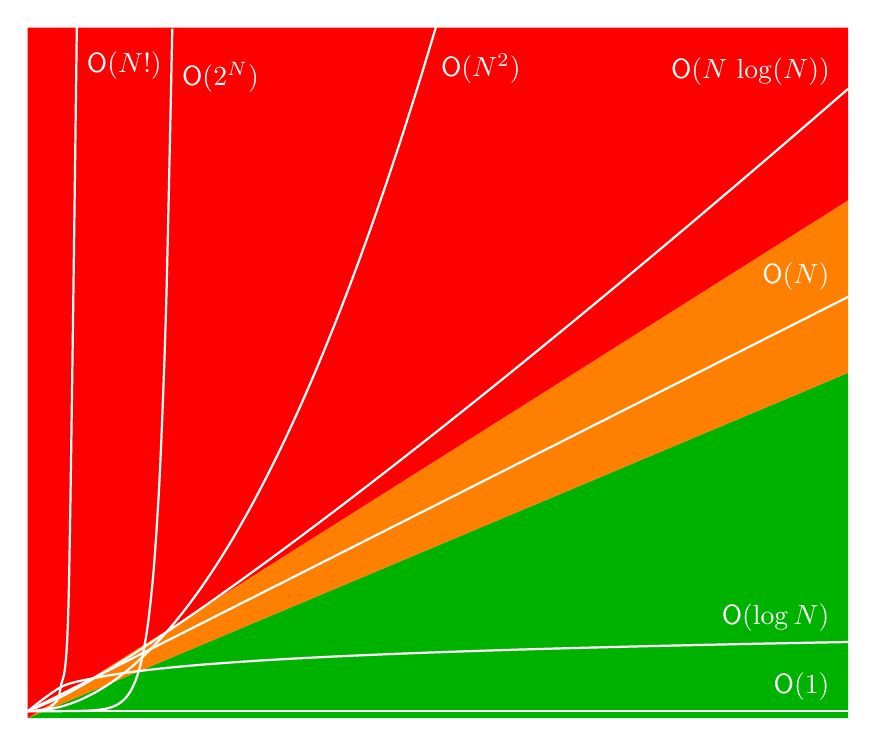
\begin{tikzpicture}
 \begin{axis}[hide axis,
    width=12cm,
    axis background/.style={path picture={
    \def\pbb{path picture bounding box}
    \fill[green!70!black] (\pbb.south west) -| (\pbb.east) -- cycle;
    \path (\pbb.east) -- (\pbb.north east) coordinate[pos=0.5] (aux);
    \fill[orange] (\pbb.south west) -- (\pbb.east) -- (aux) -- cycle;
    \fill[red] (\pbb.south west) -- (aux) -- (\pbb.north east) -| cycle;
    }},
    every axis plot/.append style={no marks,smooth,thick},
    xmin=0,xmax=100,ymin=0,ymax=100,domain=0:100]
  \addplot[white] {1} node[pos=0.99,above left]{$\mathsf{O}(1)$};   
  \addplot[white] {1+5*ln(1+x)/ln(10)} node[pos=0.99,above  left]{$\mathsf{O}(\log N)$};
  \addplot[white] {1+0.6*x} node[pos=0.99,above left]{$\mathsf{O}(N)$};     
  \addplot[white] {1+0.3*x*(1+ln(1+x)/ln(10))} node[pos=0.99,above  left]{$\mathsf{O}(N\,\log(N))$};    
  \addplot[white,domain=0:50] {1+x*x/25} node[pos=0.97,below right]{$\mathsf{O}(N^2)$};     
  \addplot[white,domain=0:17.63] {1+pow(2,x)/2048} node[pos=0.97,below  right]{$\mathsf{O}(2^N)$};  
  \addplot[white,samples at={1,2,...,6}] {1+x!*100/6!} node[pos=0.97,below  right]{$\mathsf{O}(N!)$};   
 \end{axis}
\end{tikzpicture}
\captionof{figure}{Graph of some of the most common Big O functions.}
\end{center}

Research questions:
\begin{itemize}
    \item What is the practical time complexity of every algorithms?
    \item Does it align with the theory?
    \item What are the advantages and disadvantages of every algorithm?
\end{itemize}

\section{Method}
All the algorithms have been implemented using Java v16 and they have been executed multiple times in order to mitigate the variability introduced by the operating system scheduler.
The execution time measures the minimum number of instructions needed for the algorithm to complete its job and leaves out the time used by the surrounding code.

\newpage
\section{Result}

\begin{table}[h!]
\begin{center}
\begin{tabular}{| c | c | c | r | r | r | r | r |} 
 \hline
 \multicolumn{3}{|c|}{\multirow{2}{*}{Algorithm}} & \multicolumn{5}{c|}{Input size} \\
 \cline{4-8}
 \multicolumn{3}{|c|}{} & 20 000 & 40 000 & 60 000 & 80 000 & 100 000 \\
 \hline
 \multirow{3}{*}{Quick Sort}
 & median of 3 elements pivot
 & recursive
 & 804 & 3073 & 7753 & 13186 & 19487 \\
 \cline{2-8}
 & random element pivot
 & iterative
 & 90 & 314 & 677 & 1179 & 1860 \\
 \cline{2-8}
 & first element pivot
 & recursive
 & 73 & 275 & 605 & 1065 & 1656 \\
 \hline
 Insertion Sort
 & - & iterative
 & 5541 & 15428 & 34965 & 63185 & 99659 \\ 
 \hline
 Merge Sort
 & - & recursive
 & 22 & 43 & 62 & 86 & 106 \\ 
 \hline
 Binary Search
 & - & recursive
 & 0 & 0 & 0 & 0 & 0 \\ 
 \hline
\end{tabular}
\caption{Average time in milliseconds (10 cycles) in relation to the inputs size.}
%\label{table:1}
\end{center}
\end{table}
As shown by the previous table, the execution time varies greatly, for that reason the y axis of the following plot use a logarithmic scale:
\begin{center}
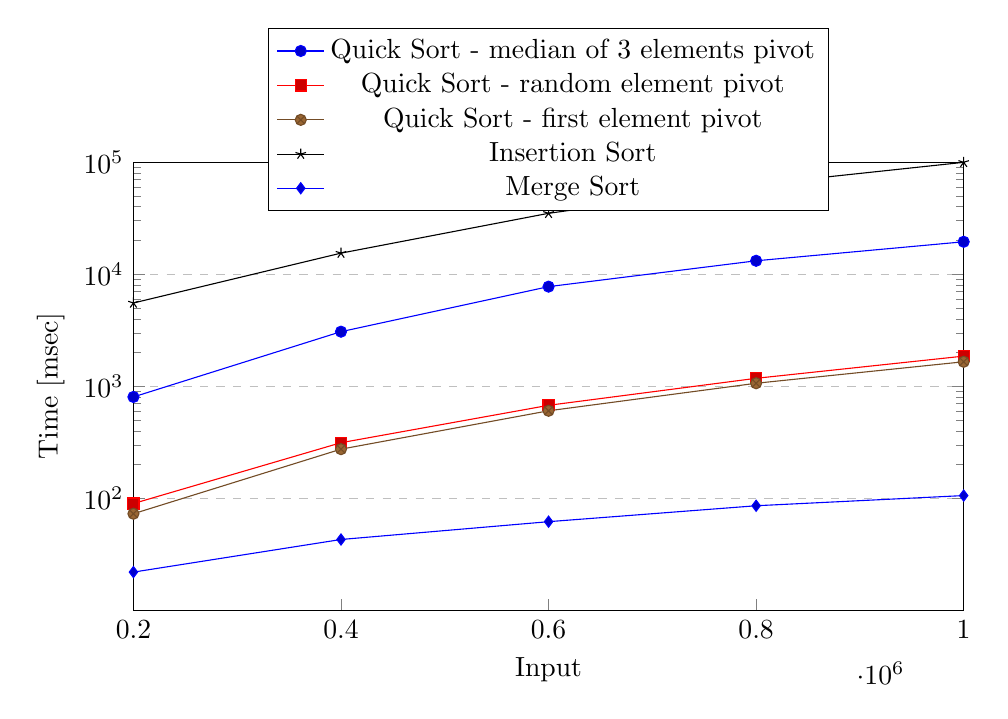
\begin{tikzpicture}
\begin{axis}[
    %title={Running times},
    width=1.0\textwidth,
    height=0.6\textwidth,
    xmode=normal,
    ymode=log,
    xlabel={Input},
    ylabel={Time [msec]},
    xmin=200000, xmax=1000000,
    ymin=10, ymax=100000,
    xtick={200000, 400000, 600000, 800000, 1000000},
    ytick={10e1, 10e2, 10e3, 10e4, 10e5},
    legend style={at={(0.5,1.3)},anchor=north},
    ymajorgrids=true,
    grid style=dashed]
\addplot
    coordinates {
    (200000,804)(400000,3073)(600000,7753)(800000,13186)(1000000,19487)
    };
\addlegendentry{Quick Sort - median of 3 elements pivot}
\addplot
    coordinates {
    (200000,90)(400000,314)(600000,677)(800000,1179)(1000000,1860)
    };
\addlegendentry{Quick Sort - random element pivot}
\addplot
    coordinates {
    (200000,73)(400000,275)(600000,605)(800000,1065)(1000000,1656)
    };
\addlegendentry{Quick Sort - first element pivot}
\addplot
    coordinates {
    (200000,5541)(400000,15428)(600000,34965)(800000,63185)(1000000,99659)
    };
\addlegendentry{Insertion Sort}
\addplot
    coordinates {
    (200000,22)(400000,43)(600000,62)(800000,86)(1000000,106)
    };
\addlegendentry{Merge Sort}
\addplot
    coordinates {
    (200000,0)(400000,0)(600000,0)(800000,0)(1000000,0)
    };
\addlegendentry{Binary Search}
\end{axis}
\end{tikzpicture}
\captionof{figure}{Running times of all the tested algorithms.}
\end{center}

\newpage
\section{Quick Sort}
\subsection{Median of 3 elements pivot}

\begin{center}
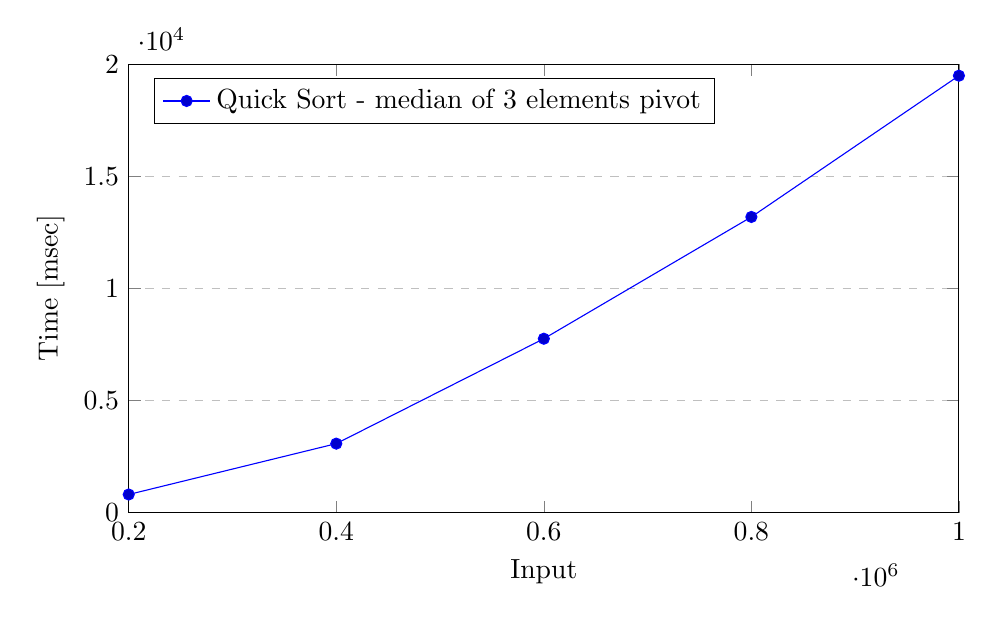
\begin{tikzpicture}
\begin{axis}[
    %title={Running times},
    width=1.0\textwidth,
    height=0.6\textwidth,
    xmode=normal,
    ymode=normal,
    xlabel={Input},
    ylabel={Time [msec]},
    xmin=200000, xmax=1000000,
    ymin=0, ymax=20000,
    xtick={200000, 400000, 600000, 800000, 1000000},
    ytick=,
    legend pos=north west,
    ymajorgrids=true,
    grid style=dashed,
    legend pos=north west]
\addplot
    coordinates {
    (200000,804)(400000,3073)(600000,7753)(800000,13186)(1000000,19487)
    };
\addlegendentry{Quick Sort - median of 3 elements pivot}
% \addplot [
%     domain=200000:1000000, 
%     samples=100, 
%     ]
%     {0.00019875*x*(log2(x))};
\end{axis}
\end{tikzpicture}
\captionof{figure}{Running times of Quick Sort - Median of 3 elements pivot.}
\end{center}

\textbf{Computation on T(N)}\\

Expected complexity: $O(NlogN)$\\

\LOG[2]{2}{\logTwoResult}
\MULTIPLY{\logTwoResult}{2}{\logTwoMultiplied}
\LOG[2]{10}{\logTenResult}
\MULTIPLY{\logTenResult}{10}{\logTenMultiplied}

\begin{enumerate}
    \MULTIPLY{804}{\logTwoMultiplied}{\resultQuickSortMedianTwoTimes}
    \item $T(400\,000) = 804 *2 log 2 = \resultQuickSortMedianTwoTimes < 3073$\\
    The algorithm is twice as fast as the worst case.
    
    % \MULTIPLY{804}{\logTenMultiplied}{\resultQuickSortMedianTenTimes}
    \item $T(1\,000\,000) = 804 *10 log 10 =$
    % \directlua{tex.print(math.floor(804*10*math.log(10, 2)))}
    $> 19487$\\
    The algorithm is slower than the theoretical worst case.
    
\end{enumerate}

\textbf{Analysis}\\

In theory this algorithm should have been the fastest implementation of QuickSort but probably due to its recursive implementation turned out to be the slowest. Recursion is usually slower than iteration because the CPU has to deal with the recursive call stack frame, in addition to processing the loop content.

\newpage
\subsection{Random element pivot}

\begin{center}
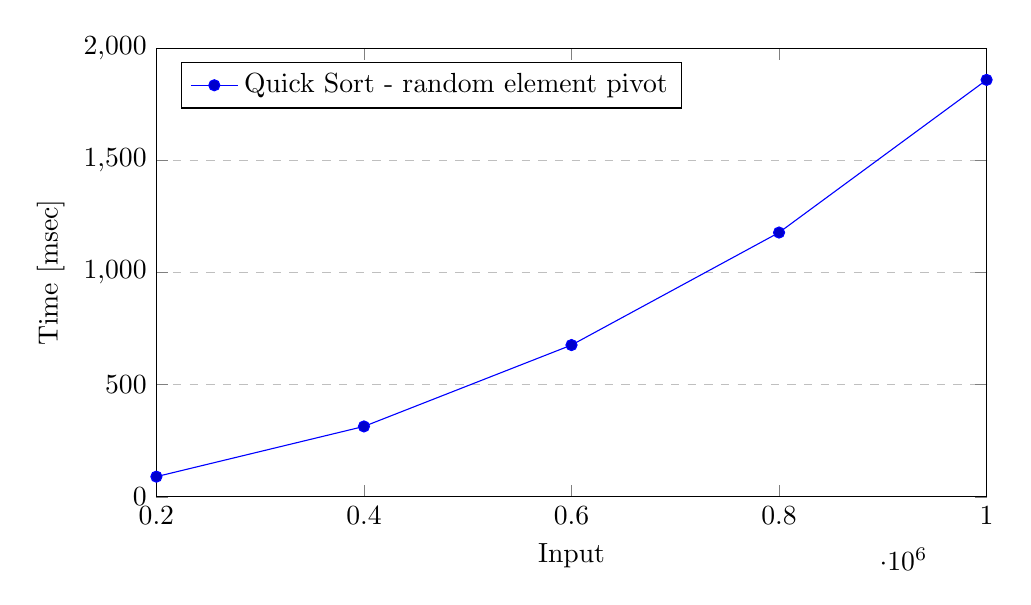
\begin{tikzpicture}
\begin{axis}[
    %title={Running times},
    width=1.0\textwidth,
    height=0.6\textwidth,
    xmode=normal,
    ymode=normal,
    xlabel={Input},
    ylabel={Time [msec]},
    xmin=200000, xmax=1000000,
    ymin=0, ymax=2000,
    xtick={200000, 400000, 600000, 800000, 1000000},
    ytick=,
    legend pos=north west,
    ymajorgrids=true,
    grid style=dashed,
    legend pos=north west]
\addplot
    coordinates {
    (200000,90)(400000,314)(600000,677)(800000,1179)(1000000,1860)
    };
\addlegendentry{Quick Sort - random element pivot}
\end{axis}
\end{tikzpicture}
\captionof{figure}{Running times of Quick Sort - Random element pivot.}
\end{center}

\textbf{Computation on T(N)}\\

Expected complexity: $O(NlogN)$\\

\begin{enumerate}
    \item $T(400\,000) = 90 *2 log 2 =$
    % \directlua{tex.print(math.floor(90*2*math.log(2, 2)))}
    $< 314$\\
    The algorithm is almost twice as fast as the worst case.
    
    % \MULTIPLY{804}{\logTenMultiplied}{\resultQuickSortMedianTenTimes}
    \item $T(1\,000\,000) = 90 *10 log 10 =$
    % \directlua{tex.print(math.floor(90*10*math.log(10, 2)))}
    $> 1860$\\
    The algorithm is slower than the theoretical worst case.
    
\end{enumerate}

\newpage
\subsection{First element pivot}

\begin{center}
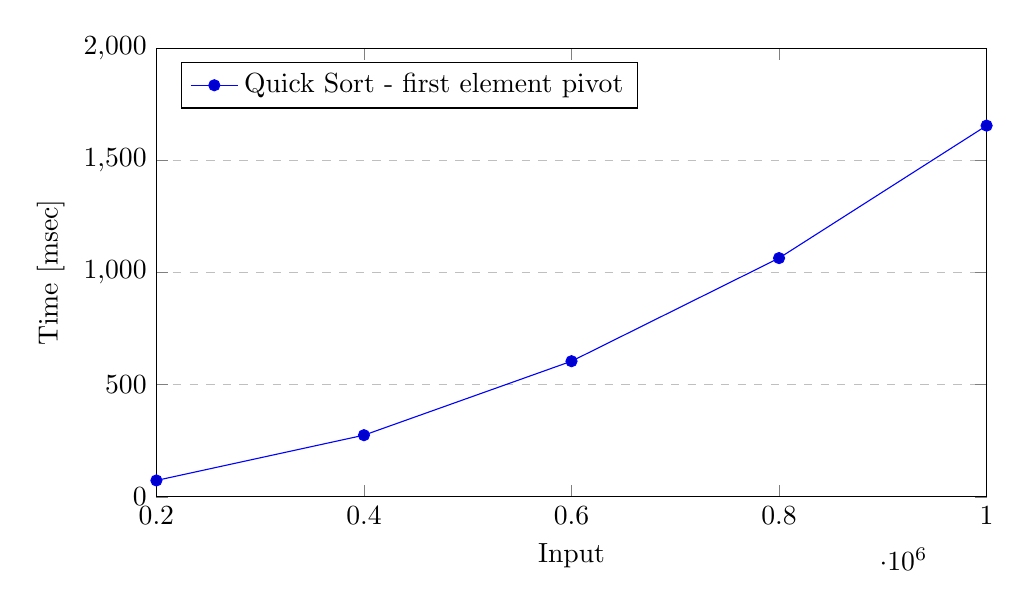
\begin{tikzpicture}
\begin{axis}[
    %title={Running times},
    width=1.0\textwidth,
    height=0.6\textwidth,
    xmode=normal,
    ymode=normal,
    xlabel={Input},
    ylabel={Time [msec]},
    xmin=200000, xmax=1000000,
    ymin=0, ymax=2000,
    xtick={200000, 400000, 600000, 800000, 1000000},
    ytick=,
    legend pos=north west,
    ymajorgrids=true,
    grid style=dashed,
    legend pos=north west]
\addplot
    coordinates {
    (200000,73)(400000,275)(600000,605)(800000,1065)(1000000,1656)
    };
\addlegendentry{Quick Sort - first element pivot}
\end{axis}
\end{tikzpicture}
\captionof{figure}{Running times of Quick Sort - First element pivot.}
\end{center}

\textbf{Computation on T(N)}\\

Expected complexity: $O(NlogN)$\\

\begin{enumerate}
    \item $T(400\,000) = 73 *2 log 2 =$
    % \directlua{tex.print(math.floor(73*2*math.log(2, 2)))}
    $< 275$\\
    The algorithm is twice as fast as the worst case.
    
    % \MULTIPLY{804}{\logTenMultiplied}{\resultQuickSortMedianTenTimes}
    \item $T(1\,000\,000) = 73 *10 log 10 =$
    % \directlua{tex.print(math.floor(73*10*math.log(10, 2)))}
    $> 1656$\\
    The algorithm is slower than the theoretical worst case.
    
\end{enumerate}

\textbf{Analysis}\\

The performance of this algorithm are extremely similar to that of QuickSort with a random element pivot. This is partially expected because both algorithm have a similar way of selecting the pivot even if one is implement in a recursive fashion and the other is iterative.

\newpage
\section{Insertion Sort}

\begin{center}
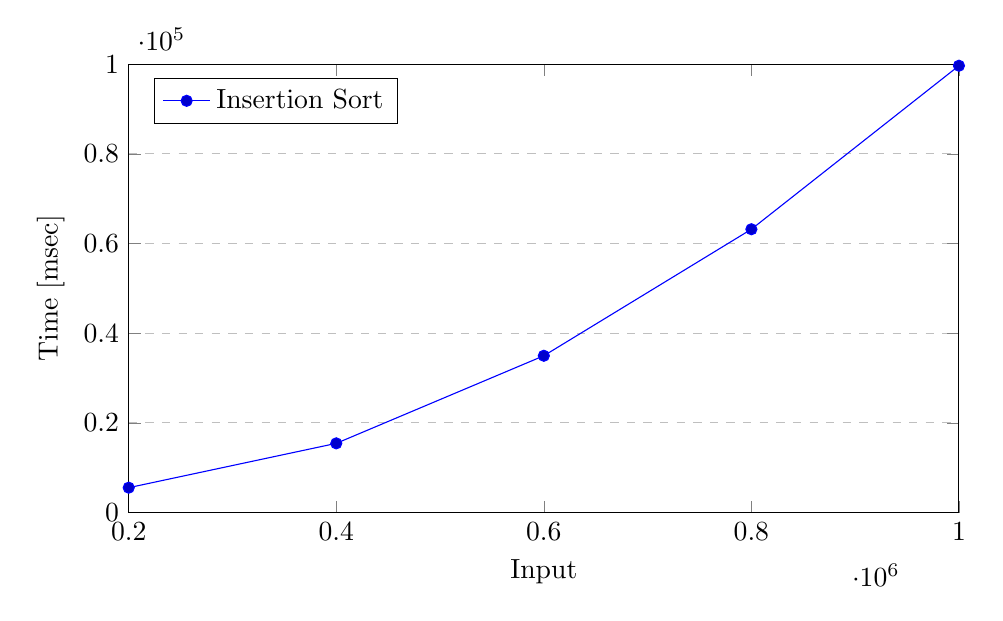
\begin{tikzpicture}
\begin{axis}[
    %title={Running times},
    width=1.0\textwidth,
    height=0.6\textwidth,
    xmode=normal,
    ymode=normal,
    xlabel={Input},
    ylabel={Time [msec]},
    xmin=200000, xmax=1000000,
    ymin=0, ymax=100000,
    xtick={200000, 400000, 600000, 800000, 1000000},
    ytick=,
    legend pos=north west,
    ymajorgrids=true,
    grid style=dashed,
    legend pos=north west]
\addplot
    coordinates {
    (200000,5541)(400000,15428)(600000,34965)(800000,63185)(1000000,99659)
    };
\addlegendentry{Insertion Sort}
\end{axis}
\end{tikzpicture}
\captionof{figure}{Running times of Insertion Sort.}
\end{center}

\textbf{Computation on T(N)}\\

Expected complexity: $O(N^2)$\\

\begin{enumerate}
    \item $T(400\,000) = 5541 *2^2 =$
    % \directlua{tex.print(math.floor(5541*2*2))}
    $> 15428$\\
    The algorithm is slower than the worst case.
    
    % \MULTIPLY{804}{\logTenMultiplied}{\resultQuickSortMedianTenTimes}
    \item $T(1\,000\,000) = 5541 *10^2 =$
    % \directlua{tex.print(math.floor(5541*10*10))}
    $> 99659$\\
    The algorithm is more than five time slower than the theoretical worst case.
    
\end{enumerate}

\textbf{Analysis}\\

As expected, Insertion Sort is the slowest algorithm  because it is better suited for small inputs or when data is nearly sorted which was not the case in this test.

\newpage
\section{Merge Sort}

\begin{center}
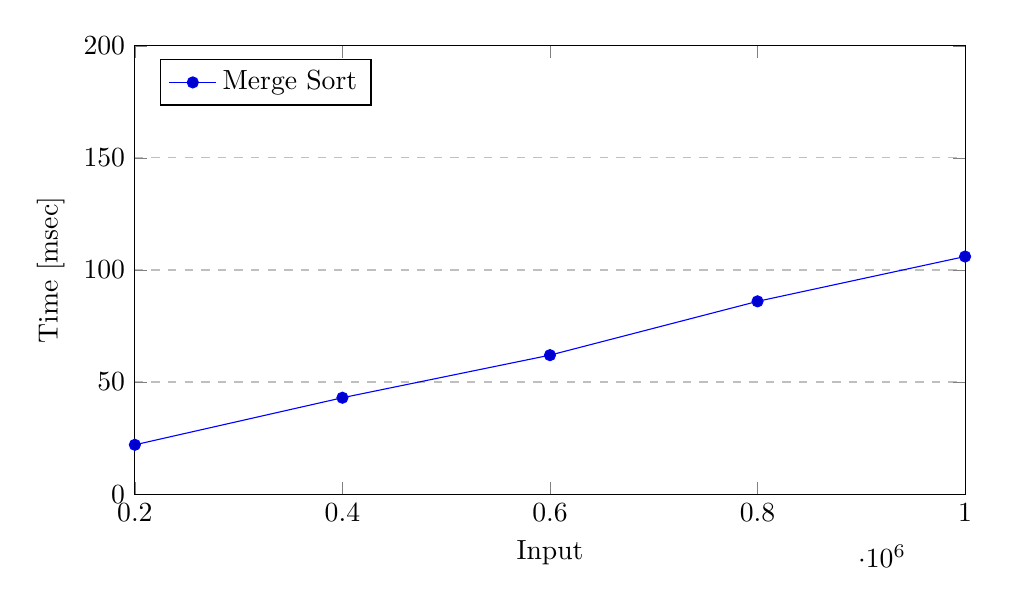
\begin{tikzpicture}
\begin{axis}[
    %title={Running times},
    width=1.0\textwidth,
    height=0.6\textwidth,
    xmode=normal,
    ymode=normal,
    xlabel={Input},
    ylabel={Time [msec]},
    xmin=200000, xmax=1000000,
    ymin=0, ymax=200,
    xtick={200000, 400000, 600000, 800000, 1000000},
    ytick=,
    legend pos=north west,
    ymajorgrids=true,
    grid style=dashed,
    legend pos=north west]
\addplot
    coordinates {
    (200000,22)(400000,43)(600000,62)(800000,86)(1000000,106)
    };
\addlegendentry{Merge Sort}
\end{axis}
\end{tikzpicture}
\captionof{figure}{Running times of Merge Sort.}
\end{center}

\textbf{Computation on T(N)}\\

Expected complexity: $O(NlogN)$\\

\begin{enumerate}
    \item $T(400\,000) = 22 *2 log 2 =$
    % \directlua{tex.print(math.floor(22*2*math.log(2, 2)))}
    $> 43$\\
    The algorithm execution time is nearly identical to the worst case.
    
    % \MULTIPLY{804}{\logTenMultiplied}{\resultQuickSortMedianTenTimes}
    \item $T(1\,000\,000) = 22 *10 log 10 =$
    % \directlua{tex.print(math.floor(22*10*math.log(10, 2)))}
    $> 106$\\
    The algorithm is slower than the theoretical worst case.
    
\end{enumerate}

\textbf{Analysis}\\

Merge Sort requires more memory space than Quick Sort but its recursive implementation is definitely the fastest.

\newpage
\section{Binary Search}

\begin{center}
\begin{tikzpicture}
\begin{axis}[
    %title={Running times},
    width=1.0\textwidth,
    height=0.6\textwidth,
    xmode=normal,
    ymode=normal,
    xlabel={Input},
    ylabel={Time [msec]},
    xmin=200000, xmax=1000000,
    ymin=0, ymax=10,
    xtick={200000, 400000, 600000, 800000, 1000000},
    ytick={},
    legend pos=north west,
    ymajorgrids=true,
    grid style=dashed,
    legend pos=north west]
\addplot
    coordinates {
    (200000,0)(400000,0)(600000,0)(800000,0)(1000000,0)
    };
\addlegendentry{Binary Search}
\end{axis}
\end{tikzpicture}
\captionof{figure}{Running times of Binary Search.}
\end{center}


\textbf{Computation on T(N)}\\

Expected complexity: $O(logN)$\\

\textbf{Analysis}\\

The implementation of Binary Search was so fast that for every input size the measured execution time was zero. Increasing the input size over 10 millions was not possible because of memory limitation on the PC used. It is nonetheless possible to conclude that its time complexity increase very slowly, most likely as predicted by the theory.

\newpage
\section{Conclusion}

Sorting algorithms are very important, useful and widely used so, finding the most efficient one for a given application can yield big benefits. Unfortunately theoretical analysis and practical implementations not always agrees thus, it is crucial to test the chosen algorithm before making a definitive choice. The specific use case and data structures that are going to be used can have a big impact on the final efficiency and mark a successful implementation from a failed one.

\newpage

\nocite{*}
\printbibliography[] % to hide showing references again

\end{document}
